\documentclass{beamer}
\usepackage{listings}

\begin{document}

\title[git]
{A short introduction to version control with Git}
\subtitle{Git - You'll never learn it all!}
\author[Blundell]
{Benjamin ~Blundell\inst{1}}
\institute[ITS Research, QMUL]
{
  \inst{1}
  ITS Research\\
  Queen Mary University of London
 }
\date[2016]
{CIS Software Engineering Day, 2016}
\subject{Computer Science}

% Slides
% Title
\frame{\titlepage}


% Introduction
\begin{frame}
  \frametitle{Introduction}
  
  \begin{block}{Me}
    \begin{itemize}  
      \item b.blundell@qmul.ac.uk 
      \item ITS Research - writing programs for scientists and artists.
      \item Helping people with their HPC problems.
      \item Previously ran small company building graphics-type things
      \item I write stuff at www.section9.co.uk
      \item I use Git everyday
    \end{itemize}
  \end{block}

\end{frame}


% What is it?
\begin{frame}
  \frametitle{What is it?}

  \begin{block}{What is git?}
    \begin{itemize}  
      \item Version control system developed for the Linux Kernel. 
      \item Distributed as opposed to centralised.
      \item A suite of many, many small tools.
    \end{itemize}
  \end{block}

  \begin{block}{What is github?}
    \begin{itemize}  
      \item Git, but on the internets.
      \item User-friendly interface including visualisations.
      \item A social network of sorts.
    \end{itemize}
  \end{block}

\end{frame}

% Why?
\begin{frame}
  \frametitle{How will Git help me right now?}

  \begin{block}{Advantages to version control}
    \begin{itemize}  
      \item Backing up your work.
      \item Undo-ing changes you've made.
      \item Sharing work with others.
    \end{itemize}
  \end{block}

  \begin{block}{Advantages to github}
    \begin{itemize}  
      \item Collaboration (showing off?).
      \item Off-site backup of code.
      \item Public accountability.
      \item Open-source contribution.
      \item A place to put all my slides so you can get them easily.
    \end{itemize}
  \end{block}

\end{frame}

% Resources
\begin{frame}
  \frametitle{Resources}

  \begin{block}{Reference material}
    \begin{itemize}
      \item https://git-scm.com/doc
      \item https://git-scm.com/book/en/v2
      \item man pages for git
    \end{itemize}
  \end{block}

  \begin{block}{Tutorials}
    \begin{itemize}  
      \item https://try.github.io/
      \item http://gitreal.codeschool.com/
    \end{itemize}
  \end{block}

  \begin{block}{Software}
   \begin{itemize}  
      \item Git for Windows.
      \item TortoiseGit.
      \item Git is built into Visual Studio and others.
    \end{itemize}

  \end{block}
\end{frame}


% Basic Commands
\begin{frame}[fragile]
  \frametitle{Lets begin (0)}

  \begin{lstlisting}[caption=setup git for windows] 
  L:\Git-2.6.4-32-bit\git-bash.exe
  git config --global http.sslverify "false"
  \end{lstlisting}

 \begin{block}{Git for Windows}
   \begin{itemize}  
      \item Git for Windows is but one version of git
      \item Same commands on Linux and MacOS
    \end{itemize}
  \end{block}


\end{frame}


% Basic Commands
\begin{frame}[fragile]
  \frametitle{Lets begin (1)}

  \begin{lstlisting}[caption=clone a repository] 
  git clone https://github.com/QMUL/gitclass.git
  git status
  \end{lstlisting}

  \begin{lstlisting}[caption=create a new repository] 
  git init 
  \end{lstlisting}

\end{frame}


% Changes
\begin{frame}[fragile]
  \frametitle{Making changes}
  
  \begin{lstlisting}[caption=Making changes] 
  git status
  git add <your filename>
  git status
  \end{lstlisting}

\end{frame}

% Changes
\begin{frame}[fragile]
  \frametitle{Differences and Reset}
  
  \begin{lstlisting}[caption=Making changes] 
  git diff --staged
  \end{lstlisting}

  \begin{lstlisting}[caption=Reset changes] 
  git reset <myfilename>
  \end{lstlisting}

\end{frame}

% Forking
\begin{frame}[fragile]
  \frametitle{Forking on Github}
  
  \begin{block}{Forking}
   \begin{itemize}  
      \item Not strictly a git command per-se. A github.com feature
      \item Creating our own version and copy online on github
      \item Related to the original
    \end{itemize}
  \end{block}

\end{frame}

% Remote
\begin{frame}[fragile]
  \frametitle{Remote Copies / Repositories}
  
  \begin{block}{Remote}
   \begin{itemize}  
      \item A copy of the repository, complete and somewhere else.
      \item Could be github, or another directory on the same disk.
    \end{itemize}
  \end{block}

  \begin{lstlisting}[caption=Reset changes] 
  git remote add cis <address>
  git@github.com:MYUSERNAME/gitclass.git
  git remote --help
  \end{lstlisting}

\end{frame}

% Commit
\begin{frame}[fragile]
  \frametitle{Committing changes}
  
  \begin{block}{commit}
    \begin{itemize}  
      \item Possibly the most used command
      \item Staged changes are 'committed'.
    \end{itemize}
  \end{block}

  \begin{lstlisting}[caption=git commit] 
  git commit --help
  git commit -a -m "<my message>"
  \end{lstlisting}

\end{frame}

% Push

\begin{frame}[fragile]
  \frametitle{Pushing Commits}
  
  \begin{block}{push}
    \begin{itemize}  
      \item Pushing your commits to a remote repository.
    \end{itemize}
  \end{block}

  \begin{lstlisting}[caption=git push] 
  git push cis master
  git diff
  \end{lstlisting}
\end{frame}

% Log
\begin{frame}[fragile]
  \frametitle{Checking History}
  
  \begin{block}{checking}
    \begin{itemize}  
      \item Looking at the history of commits
      \item List of git commit messages and unique IDs
    \end{itemize}
  \end{block}

  \begin{lstlisting}[caption=git log] 
  git log
  \end{lstlisting}
\end{frame}

% Removing things

\begin{frame}[fragile]
  \frametitle{Removing files}
  
  \begin{lstlisting}[caption=Removing Files] 
  git rm <your file name>
  git commit -a -m "removed our new file"
  \end{lstlisting}

\end{frame}

% Undoing things

\begin{frame}[fragile]
  \frametitle{Its all gone wrong(0)}

  \begin{block}{wrong}
   \begin{itemize}  
      \item What do we do if we delete or change things and we want to go back
      \item We need to think about pointers and commit IDs
    \end{itemize}
  \end{block}

  \begin{block}{Pointers}
    \includegraphics[height=3cm]{branch-and-history.png}
  \end{block}


\end{frame}


\begin{frame}[fragile]
  \frametitle{Its all gone wrong(1)}
  
  \begin{lstlisting}[caption=restoring things] 
  git reset --hard HEAD~1
  git reset --hard HEAD
  \end{lstlisting}

\end{frame}

% Branching

\begin{frame}[fragile]
  \frametitle{Branching (0)}

  \begin{block}{branching}
   \begin{itemize}  
      \item Probably the heart of Git - different code with a common history.
      \item Can 'branch off' from the main codebase to test things.
      \item Can merge back at a later date. Everything recorded.
    \end{itemize}
  \end{block}

  \begin{block}{master and testing branches}
    \includegraphics[height=3cm]{advance-master.png}
  \end{block}


\end{frame}

\begin{frame}[fragile]
  \frametitle{Branching (1)}

  \begin{lstlisting}[caption=branching] 
  git branch morespeare
  git branch
  \end{lstlisting}

  \begin{lstlisting}[caption=make some changes] 
  https://archive.org/details/
    gutenberg?and[]=shakespeare
  
  git commit -a -m "Added more shakespeare to use"
  git push origin morespeare
  \end{lstlisting}


\end{frame}

\begin{frame}[fragile]
  \frametitle{Merging}

  \begin{block}{Merging}
   \begin{itemize}  
      \item The counterpart to branching.
      \item The trick is to recognise and resolve conflicts
    \end{itemize}
  \end{block}

  \begin{lstlisting}[caption=make some changes] 
  git checkout master 
  git merge morespeare
  \end{lstlisting}

\end{frame}


\begin{frame}[fragile]
  \frametitle{Conflicts}

  \begin{lstlisting}[caption=possible result of a merge] 
  Auto-merging shakespeare_corpus.txt
  CONFLICT (content): Merge conflict in shakespeare_corpus.txt
  Automatic merge failed; fix conflicts and then commit the result.
  \end{lstlisting}

 \begin{lstlisting}[caption=a conflict] 
  <<<<<<< HEAD:index.html
  <div id="footer">contact : email.support@github.com</div>
  =======
  <div id="footer">
  please contact us at support@github.com
  </div>
  >>>>>>> iss53:index.html
 \end{lstlisting}

\end{frame}

% Collaboration

\begin{frame}[fragile]
  \frametitle{Collaboration}
  Using remote repositories with correct access controls we can work collaboratively.
 
  \begin{block}{collaboration}
   \begin{itemize}  
      \item github.com is perhaps the most widely known.
      \item git-lab.
      \item gitolite with keys and a server.
      \item Any remote repository where you can get access.
    \end{itemize}
  \end{block}

 

\end{frame}


\begin{frame}[fragile]
  \frametitle{Advanced Topics}
  Practical Exercise before we move onto advanced topics.
\end{frame}


% Advanced Topics

% stashing

\begin{frame}[fragile]
  \frametitle{Stashing}
  Sometimes you want to temporarily store changes and come back to them later without commiting.

  \begin{lstlisting}[caption=stashing] 
  git stash
  git status
  git stash list
  git stash apply
  \end{lstlisting}

\end{frame}

% rebasing

\begin{frame}
  \frametitle{rebasing}
    Rebasing, in some ways, is another way to perform a merge (amongst other things). It *replays* changes on-top of a common ancestor.

  \begin{block}{example with merging}
    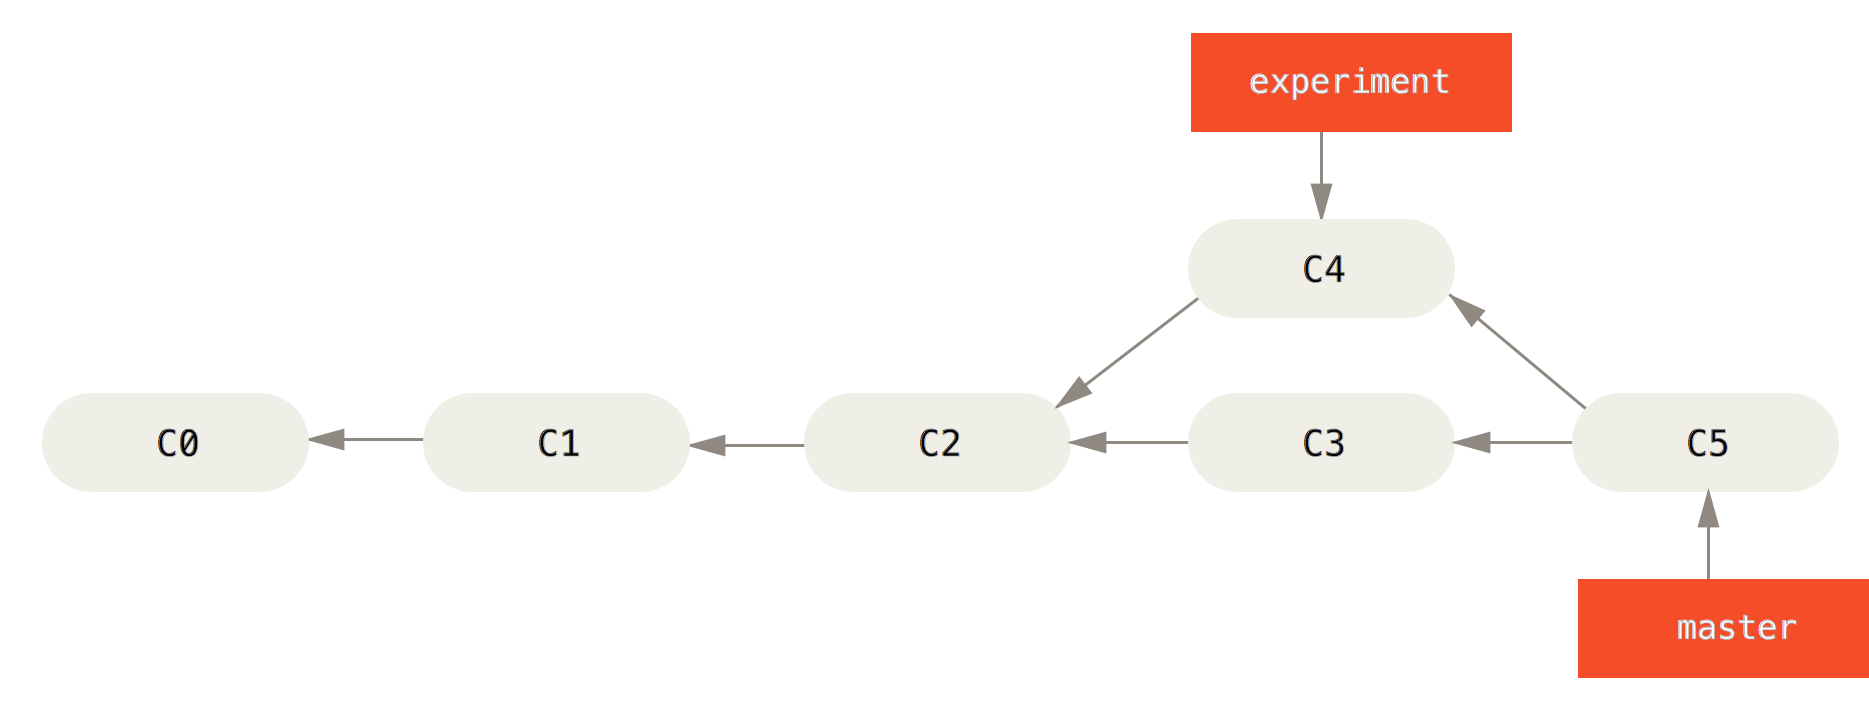
\includegraphics[height=3cm]{basic-rebase-2.png}
  \end{block}

\end{frame}

\begin{frame}[fragile]
  \frametitle{rebasing 2}
  
  \begin{lstlisting}[caption=rebase] 
   git checkout experiment
   git rebase master
  \end{lstlisting}

  \begin{block}{example with a rebase}
    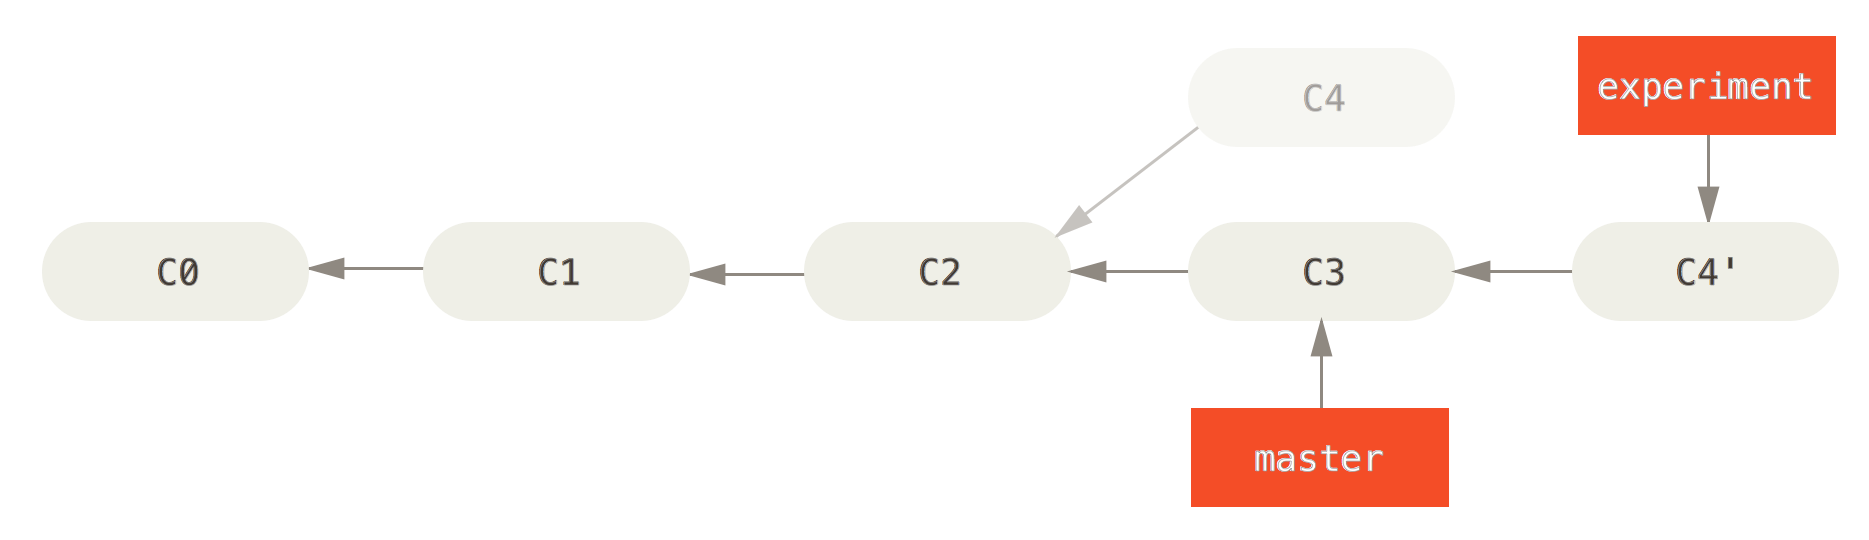
\includegraphics[height=3cm]{basic-rebase-3.png}
  \end{block}

\end{frame}

\begin{frame}[fragile]
  \frametitle{rebasing 3}
  
  \begin{lstlisting}[caption=rebase] 
    git checkout master
    git merge experiment
  \end{lstlisting}

  \begin{block}{example with a rebase}
    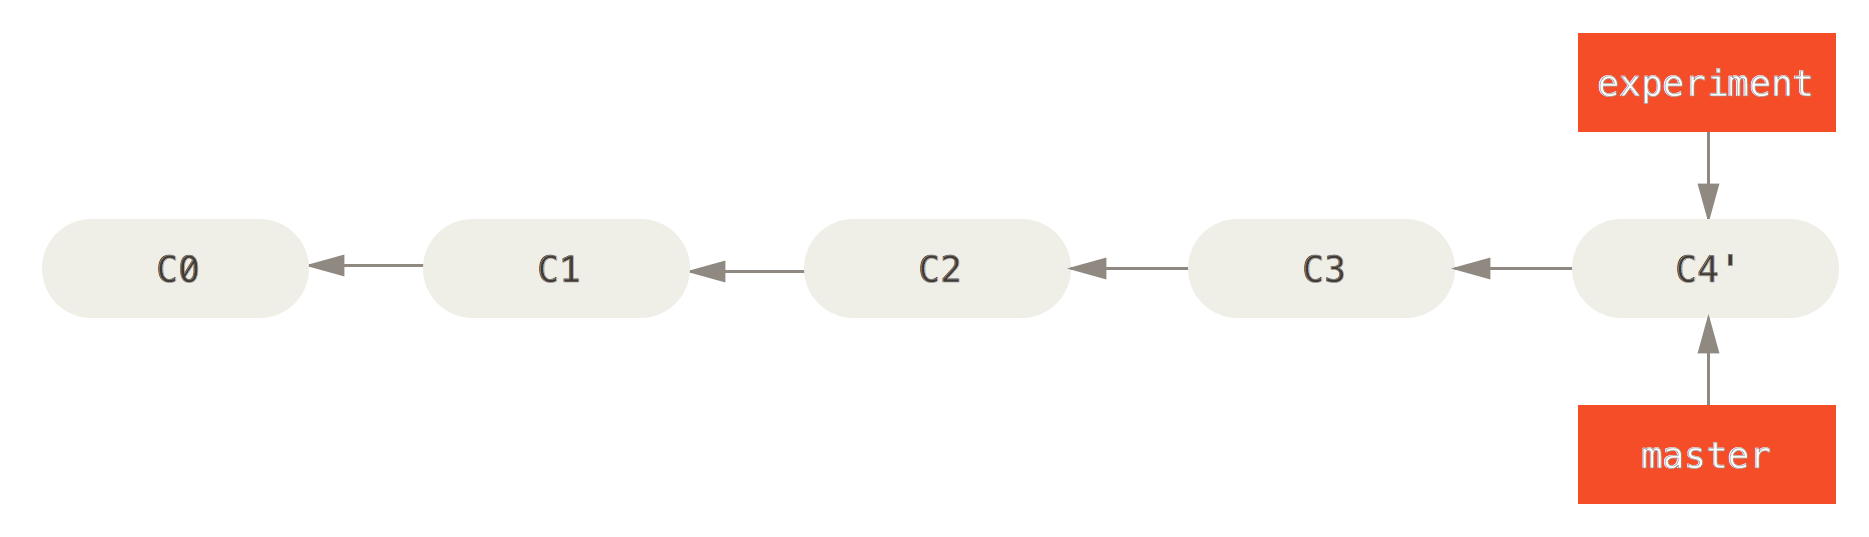
\includegraphics[height=3cm]{basic-rebase-4.png}
  \end{block}

\end{frame}


% tagging

\begin{frame}[fragile]
  \frametitle{tagging}
  Tags are good ways to mark commits. Also useful for people when they checkout your code. 

  \begin{lstlisting}[caption=tagging] 
   git tag
   git tag -a v1.4 -m "my version 1.4"
   git show v1.4
  \end{lstlisting}

  Can create lightweight tags (just the checksum) by not adding -a.

\end{frame}

% diffing

\begin{frame}[fragile]
  \frametitle{diff}
  Tools to see the differences and create patches from these differences.

  \begin{lstlisting}[caption=diff examples] 
   git diff
   git diff HEAD
   git diff HEAD^ HEAD
  \end{lstlisting}

  Various other tools like vimdiff, and more advanced diffs across branches

  \begin{lstlisting}[caption=diff examples 2] 
    git difftool --tool=vimdiff --no-prompt \
      origin/togusa:.vimrc .vimrc
  \end{lstlisting}

\end{frame}

% Flows

\begin{frame}
  \frametitle{Flows}
  A way to organise your work. Use branches and tags to keep work organised. 
 
  \begin{itemize}
    \item development/trunk
    \item stage/pre-production
    \item production/live
  \end{itemize}
 
\end{frame}

% Build Systems

\begin{frame}
  \frametitle{Integrating Git with workflow}
  Git and github work well with other tools. Automatic build-tools  

  \begin{itemize} 
    \item https://travis-ci.org/
    \item https://jenkins.io/index.html
  \end{itemize}
 
\end{frame}

% segue into testing

\begin{frame}
  \frametitle{Integrating Git with workflow 2}
  Can also automatically test code upon commit ... 

\end{frame}


\end{document}

